\documentclass[11pt,a4paper]{article}

\usepackage{fullpage}
\usepackage{hyperref}
\usepackage{graphicx}
\usepackage{caption}
\usepackage{subcaption}
\usepackage{graphics} 


\usepackage{fancyhdr}
\pagestyle{fancy}
\fancyhf{}
\usepackage{todonotes}

\renewcommand{\headrulewidth}{0pt}
\renewcommand{\footrulewidth}{0pt}


\begin{document}
\fancyhead[C]{special Plot: max tp table chapter 3}\begin{figure}
	\begin{subfigure}[t]{.5\textwidth}
		\centering
		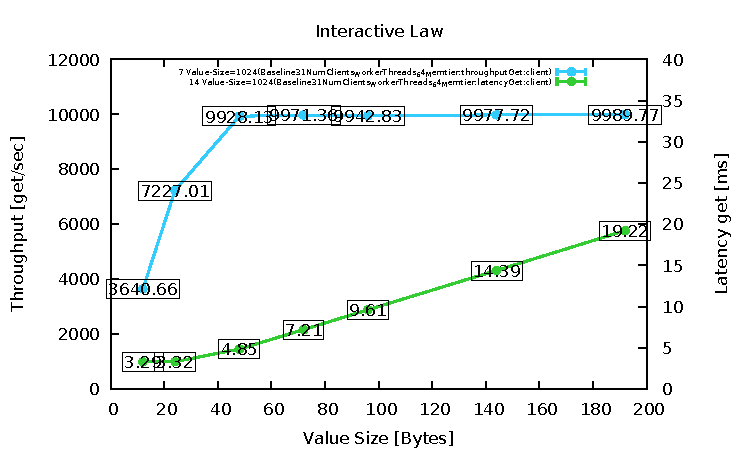
\includegraphics[width=\linewidth]{/home/fimeier/asl-fall19-project/dataSource/azure_5_12_complete/experiments/generatedPlots/allLines/pdfSource/Baseline31Client.pdf}
		\caption{Baseline31Client}
	\end{subfigure}
	\hfill
\begin{subfigure}[t]{0.5\textwidth}
		\centering
		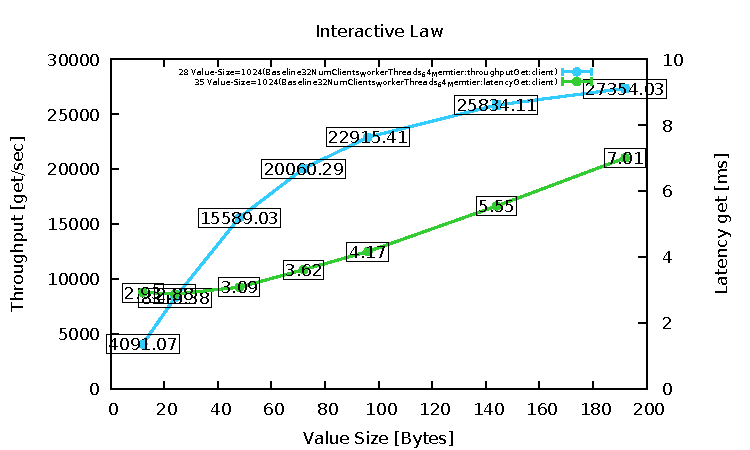
\includegraphics[width=\linewidth]{/home/fimeier/asl-fall19-project/dataSource/azure_5_12_complete/experiments/generatedPlots/allLines/pdfSource/Baseline32Client.pdf}
		\caption{Baseline32Client}
	\end{subfigure}
	
	\medskip
	\begin{subfigure}[t]{.5\textwidth}
		\centering
		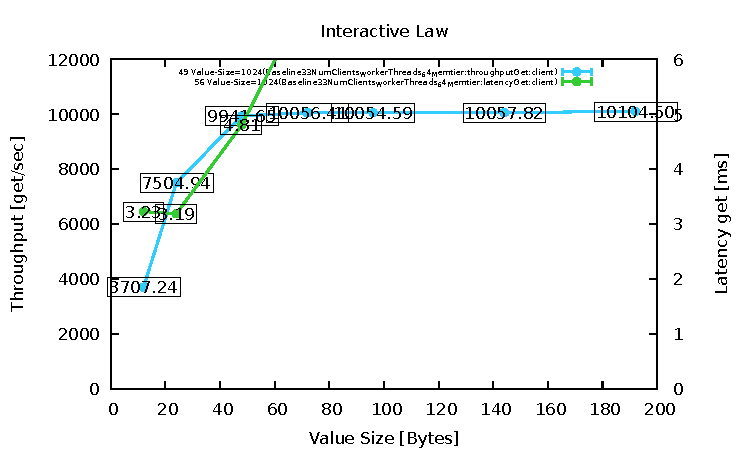
\includegraphics[width=\linewidth]{/home/fimeier/asl-fall19-project/dataSource/azure_5_12_complete/experiments/generatedPlots/allLines/pdfSource/Baseline33Client.pdf}
		\caption{Baseline33Client}
	\end{subfigure}
	\hfill
\begin{subfigure}[t]{.5\textwidth}
		\centering
		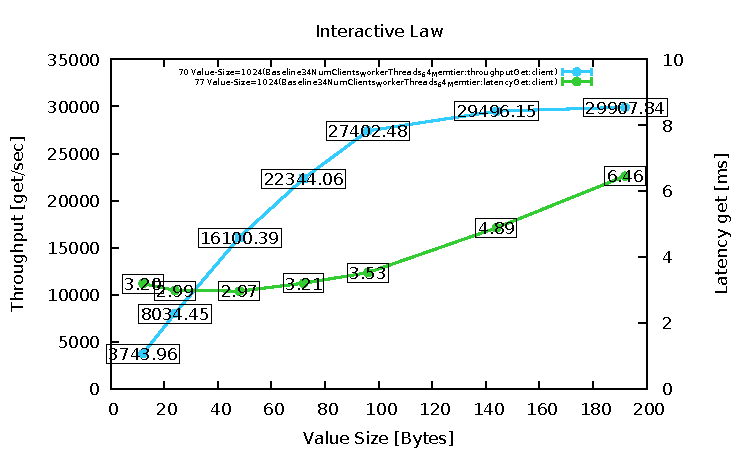
\includegraphics[width=\linewidth]{/home/fimeier/asl-fall19-project/dataSource/azure_5_12_complete/experiments/generatedPlots/allLines/pdfSource/Baseline34Client.pdf}
		\caption{Baseline34Client}
	\end{subfigure}
	
	\medskip
\end{figure}
\end{document}
